\section{Kriptografi}
  Kriptografi adalah sebuah ilmu yang mempelajari cara pengiriman pesan sehingga tidak memungkinkan bagi pihak ketiga untuk membaca ataupun memanipulasi isi pesan tersebut. Kriptografi sudah digunakan sejak jaman kerajaan Romawi Kuno dengan digunakannya Caesar Cipher oleh Julius Caesar untuk berkomunikasi dengan Jendral Perangnya. Kriptografi modern berfokus pada teori matematis dan kesulitan pihak ketiga dalam membaca atau memanipulasi pesan secara komputasional.

  Pada berbagai literatur kriptografi sering dikenal beberapa istilah seperti:
  \begin{itemize}
    \item \textit{sender}, yaitu pihak pengirim pesan
    \item \textit{receiver}, yaitu pihak penerima pesan
    \item \textit{eavesdropper}, yaitu pihak ketiga yang berusaha membaca atau memodifikasi pesan yang dikirim
    \item \textit{plaintext}, yaitu pesan yang dikirim. \textit{Plaintext} tidak harus merupakan sebuah teks namun dapat berupa audio, gambar, ataupun file binary.
    \item \textit{ciphertext}, yaitu pesan yang telah diubah oleh algoritma tertentu
    \item enkripsi, yaitu proses pengubahan \textit{plaintext} menjadi \textit{ciphertext}
    \item dekripsi, yaitu proses pengubahan \textit{ciphertext} menjadi \textit{plaintext}
    \item \textit{key}, yaitu nilai yang digunakan dalam enkripsi ataupun dekripsi
  \end{itemize}

  Pada umumnya, proses yang terjadi dalam penggunaan kriptografi pada sebuah pengiriman sebuah data dapat dilihat pada Gambar ~\ref{fig:krypto_system}:

  \begin{figure}[h]
    \centering
    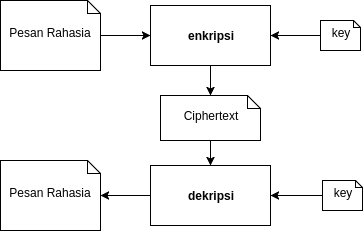
\includegraphics[width=0.6\textwidth]{resources/ch-2/crypto-system.jpg}
    \caption{Sistem pengiriman data menggunakan kriptografi}
    \label{fig:krypto_system}
  \end{figure}

  Terdapat dua macam tipe kriptografi yang saat ini umum digunakan. Kriptografi kunci simetri adalah sebuah sistem kriptografi dimana proses enkripsi dan dekripsi menggunakan kunci yang sama. Kriptografi kunci publik merupakan sebuah sistem kriptografi dimana proses enkripsi dan dekripsi menggunakan dua kunci yang berbeda.

  Masalah utama yang dihadapi pada sistem kriptografi kunci simetri adalah bagaimana dua pihak dapat menentukan sebuah kunci yang akan digunakan tanpa sepengetahuan pihak ketiga. Pada algoritma kriptografi modern, terdapat beberapa metode untuk mengirimkan kunci simetri pada pihak lain, diantaranya adalah mendekripsi key tersebut dengan algoritma kriptografi kunci publik atau dengan menggunakan algoritma \textit{key exchange}.

  \subsection{Kriptografi Kunci Publik}

    Kriptografi kunci publik adalah sebuah sistem kriptografi dimana proses enkripsi dan dekripsi dilakukan dengan kunci yang berbeda. Umumnya terdapat dua macam kunci yang terdapat pada sistem ini, yaitu \textit{public key} yang dapat dipublikasikan kepada siapapun dan \textit{private key} yang hanya dimiliki oleh pemilik kunci tersebut. \textit{Public key} digunakan untuk mengenkripsi data, sementara \textit{private key} digunakan oleh pemilik kunci untuk mendekripsi data tersebut.

    Salah satu kebutuhan utama yang terdapat pada kriptografi kunci publik adalah sebuah algoritma yang mudah untuk diproses dalam satu arah, namun sulit untuk dilakukan sebaliknya. Algoritma yang banyak digunakan umumnya berdasar pada masalah matematis seperti faktorisasi bilangan bulat, logaritma diskrit, atau hubungan kurva eliptik. Sebagai contoh, jika kita memiliki dua bilangan bulat maka dapat dengan mudah mengkalikan dua bilangan tesebut dan mendapat satu bilangan bulat baru; namun kita tidak bisa dengan mudah menentukan dua bilangan bulat yang merupakan faktor dari sebuah bilangan bulat.

    Namun, saat ini komputasi kriptografi kunci publik masih memerlukan proses komputasi yang lebih tinggi dibandingkan dengan kriptografi kunci simetris. Maka dari itu, kriptografi kunci publik biasanya hanya dilakukan untuk mengenkripsikan kunci yang akan digunakan dalam kriptografi kunci simetris.

    \subsubsection{Rivest–Shamir–Adleman (RSA)}

    RSA merupakan salah satu algoritma kriptografi kunci publik yang hingga saat ini banyak digunakan. Algoritma RSA pertama kali dicetuskan oleh Ron Rivest, Adi Shamir, dan Leonard Adleman pada tahun 1978. RSA berdasar pada sifat matematis bahwa dalam sebuah pemangkatan modular dengan persamaan:
    \begin{equation}
      (m^e)^d  \equiv  m \pmod{n}
    \end{equation}

    Pencarian tiga bilangan bulat n, e, dan d dapat dilakukan dengan mudah; bahkan untuk bilangan n, e, dan d yang sangat besar. Namun, pencarian bilangan d akan susah dilakukan, bahkan jika kita mengetahui bilangan-bilangan lainnya. Selain itu mengingat operasi perpangkatan dapat ditukar, maka proses enkripsi dan dekripsi dapat dilakukan dengan metode yang sama, hanya menggunakan bilangan yang berbeda.

    Terdapat beberapa proses yang terjadi pada algoritma RSA yaitu pembuatan \textit{public} dan \textit{private key}, distribusi \textit{public key}, enkripsi, serta dekripsi. Proses pembuatan public dan private key sendiri dilakukan dalam beberapa tahap yaitu:

    \begin{enumerate}
      \item Pilih dua bilangan prima yang besar, $p$ dan $q$.
      \item Hitung $n = p*q$ dan $ \phi = (p-1)*(q-1)$ .
      \item Pilih sebuah bilangan bulat random $e$ dengan $ 1 < e < \phi$ dan .
      \item Hitung bilangan bulat $d$, dengan $ e*d  \equiv  1 \pmod{\phi} $
    \end{enumerate}

    Dari perhitungan diatas, didapat \textit{public key} $(e, n)$ dan private key $d$.
    Proses enkripsi pada sebuah data \textit{D} dapat dilakukan melalui beberapa langkah sebagai berikut:
    \begin{enumerate}
      \item Ubah \textit{D} menjadi satu atau beberapa bilangan bulat \textit{m}, dengan \textit{m} berada dalam interval [1..n-1]
      \item Hitung ciphertext \textit{c} untuk masing-masing \textit{m}, dengan $c = m^e \bmod n $
    \end{enumerate}
